% Copyright 2004 by Till Tantau <tantau@users.sourceforge.net>.
%
% In principle, this file can be redistributed and/or modified under
% the terms of the GNU Public License, version 2.
%
% However, this file is supposed to be a template to be modified
% for your own needs. For this reason, if you use this file as a
% template and not specifically distribute it as part of a another
% package/program, I grant the extra permission to freely copy and
% modify this file as you see fit and even to delete this copyright
% notice. 

\documentclass[aspectratio=169]{beamer}

\usepackage[utf8x]{inputenc}
\usepackage[russian]{babel}

% There are many different themes available for Beamer. A comprehensive
% list with examples is given here:
% http://deic.uab.es/~iblanes/beamer_gallery/index_by_theme.html
% You can uncomment the themes below if you would like to use a different
% one:
%\usetheme{AnnArbor}
%\usetheme{Antibes}
%\usetheme{Bergen}
%\usetheme{Berkeley}
\usetheme{Berlin}
%\usetheme{Boadilla}
%\usetheme{boxes}
%\usetheme{CambridgeUS}
%\usetheme{Copenhagen}
%\usetheme{Darmstadt}
%\usetheme{default}
%\usetheme{Frankfurt}
%\usetheme{Goettingen}
%\usetheme{Hannover}
%\usetheme{Ilmenau}
%\usetheme{JuanLesPins}
%\usetheme{Luebeck}
%\usetheme{Madrid}
%\usetheme{Malmoe}
%\usetheme{Marburg}
%\usetheme{Montpellier}
%\usetheme{PaloAlto}
%\usetheme{Pittsburgh}
%\usetheme{Rochester}
%\usetheme{Singapore}
%\usetheme{Szeged}
%\usetheme{Warsaw}

\title{Презентация к Госэкзамену}

\author{Луничкин~Е.В.}
% - Give the names in the same order as the appear in the paper.
% - Use the \inst{?} command only if the authors have different
%   affiliation.

\institute[] % (optional, but mostly needed)
{
  Московский физико-технический институт (государственный университет)}
% - Use the \inst command only if there are several affiliations.
% - Keep it simple, no one is interested in your street address.

\date{Москва~--~2019}
% - Either use conference name or its abbreviation.
% - Not really informative to the audience, more for people (including
%   yourself) who are reading the slides online

\subject{Theoretical Computer Science}
% This is only inserted into the PDF information catalog. Can be left
% out. 

% If you have a file called "university-logo-filename.xxx", where xxx
% is a graphic format that can be processed by latex or pdflatex,
% resp., then you can add a logo as follows:

\pgfdeclareimage[height=0.5cm]{university-logo}{mipt_logo}
\logo{\pgfuseimage{university-logo}}

% Let's get started
\begin{document}

\begin{frame}
  \titlepage
\end{frame}

\begin{frame}{Содержание}
  \tableofcontents
  % You might wish to add the option [pausesections]
\end{frame}

% Section and subsections will appear in the presentation overview
% and table of contents.
\section{История создания КИС в США, СССР, России}

\begin{frame}
\begin{center}
  \Huge{История создания КИС в США, СССР, России. Развитие КИС: этапы,
терминология. Структура базовых КИС. Современное состояние базовых
КИС. Тенденции развития}
\end{center}
\end{frame}

\begin{frame}{История развития КИС (1/4)}
  \begin{itemize}
  \item {
    \textbf{1904-49 гг., теория}~-- принципы организации производства, заложенные Ф.~У.~Тейлором (F.~W.~Taylor, 1856-1915), пока без аппаратно-программной реализации (в силу <<неизобретённости>> и неразвитости вычислительной техники).
  }
  \item {
    \textbf{1950-64 гг., IC/IM (MRP 0)}~-- оптимизация складских запасов (Inventory Control/Management, IC/IM), расчёт и планирование потребностей в материалах (Material Requirements Planning, условно MRP 0) по Дж.~Орлики (J.~Orlicky) и О.~Уайту (O.~Wight).
  }
  \item {
    \textbf{1965-74 гг., MRP}~-- планирование потребностей в материалах (Material Requirements Planning, MRP или MRP 1), в том числе по замкнутому циклу (Closed Loop MRP), включающее составление производственной программы и ее контроль на цеховом уровне по Дж.~Дж.~Миллеру (J.~G.~Miller) и Л.~Дж.~Спраг (L.~G.~Sprague).
  }
  \end{itemize}
\end{frame}

\begin{frame}{История развития КИС (2/4)}
  \begin{itemize}
    \item {
    \textbf{1975-80 гг., MRP 2}~-- планирование производственных ресурсов (Manufacturing Resources Planning, MRP 2) на основе данных, полученных от поставщиков и потребителей, включая прогнозирование, планирование (в том числе загрузки производственных мощностей) и контроль за производством.
  }
  \item {
    \textbf{1981-85 гг., CALS}~-- добавление к MRP 2 идеологии <<точно в срок>> (Just-In-Time, JIT), элементов системы <<канбан>> (kanji + ban~-- визуальных карточек) по Ш.~Шинго (S.~Shingo) и Т.~Оно (T.~Ohno), оптимальной технологии производства (Optimized Production Technology, OPT) и оптимизации «узких мест» по Э.~Голдратту (E.~Goldratt); автоматизированная поддержка поставок (Computer-Aided Logistic Support, CALS).
  }
  \end{itemize}
\end{frame}

\begin{frame}{История развития КИС (3/4)}
  \begin{itemize}
    \item {
    \textbf{1986-90 гг., ERP}~-- планирование (всех) ресурсов предприятия (Enterprise Resources Planning, ERP), в том числе человеческих (Human Resources Management, HRM) и финансовых (Financial Resources Planning, FRP).
  }
  \item {
    \textbf{1991-96 гг., SCM, CALS 2}~-- добавление к ERP планирования ресурсов для распределения (Distribution Resources Planning, DRP); управление цепочками поставок (Supply Chain Management, SCM), позволяющее направлять и контролировать движение материальных и информационных потоков от поставщика к потребителю, по всей цепочке; непрерывная поддержка поставок и жизненного цикла (Continuous Acquisition and Lifecycle Support , CALS 2).
  }
  \end{itemize}
\end{frame}

\begin{frame}{История развития КИС (4/4)}
  \begin{itemize}
  \item {
    \textbf{1997-2000 гг., CSRP}~-- планирование ресурсов, синхронизированное с потребителями (Customer-Synchronized Resources Planning, CSRP): интегрирование потребителей и связанных с ними подразделений с основными плановыми и производственными подразделениями, интеграция собственных информационных систем с приложениями потребителей, планирование заказов потребителей.
  }
  \end{itemize}
\end{frame}

\begin{frame}{Структура базовых КИС (1/2)}
  \begin{enumerate}
  \item {
    информационная модель - представляющая собой отражение реальной информационной базы банка иописывающая все существующие информационные потоки, совокупность правил и алгоритмов функционирования информационной системы;
  }
  \item {
    техническое обеспечение (суперкомпьютеры, имеющие перспективные архитектуры и технологии организации вычислительного процесса);
  }
  \item {
    средства коммуникации (сетевые компьютерные технологии, технологии Internet/Intranet, технологии клиент~-- сервер);
  }
  \end{itemize}
\end{frame}

\begin{frame}{Структура базовых КИС (2/2)}
  \begin{enumerate}
  \setcounter{enumi}{3}
  \item {
    системное и сетевое программное обеспечение, обеспечивающее работу коммуникационных средств;
  }
  \item {
    прикладное программное обеспечение, необходимое для выполнения прикладных задач в каждом подразделении банка;
  }
  \item {
    средства обеспечения безопасности (разграничение доступа к ресурсам, обеспечение надежности функционирования корпоративной системы в целом)
  }
  \end{itemize}
\end{frame}

\begin{frame}{Современное состояние базовых КИС. Тенденции (1/2)}
  \begin{itemize}
  \item {
    Основные игроки на рынке КИС - Oracle и IBM.
  }
  \item {
    ERP-системы обрастают огромным количеством модулей.
  }
  \item {
    Используются современные алгоритмы машинного обучения для построения BI-систем.
  }
  \end{itemize}
\end{frame}

\begin{frame}{Современное состояние базовых КИС. Тенденции (2/2)}
  \begin{itemize}
  \item {
    Создание продвинутой аналитики действий пользователей.
  }
  \item {
    Построение рекомендательных моделей.
  }
  \item {
    Усиление рыночных позиций разработчиков КИС через приобретение сторонних компаний.
  }
  \item {
    Переход от клиент-серверных моделей КИС к модели с <<тонким клиентом>>.
  }
  \item {
    Web-центризм, то есть интернет-ориентированность всех модулей КИС.
  }
  \end{itemize}
\end{frame}

\section{ВФР}

\begin{frame}
\begin{center}
  \Huge{Выборочные функции распределения и моменты}
\end{center}
\end{frame}

\begin{frame}{Немного о временных рядах (1/2)}
  \begin{itemize}
  \item {
    Временной ряд~-- результат наблюдения за некоторой величиной $x(t)$, где $t_1, ..., t_n$~-- моменты наблюдения, $x_1, ..., x_n$~-- наблюдаемые значения величины.
  }
  \item {
    Случайный процесс~-- семейство $\{x(t), t \in T\}$. Если $t$ принимает дискретные значения, то это временной ряд.
  }
  \end{itemize}
\end{frame}

\begin{frame}{Немного о временных рядах (2/2)}
  \begin{itemize}
  \item {
    Непрерывная случайная величина $\xi$ принимает дискретное множество значений, если наблюдается в дискретные моменты времени.
  }
  \item {
    Распределением дискретной случайной величины $\xi$ называется множество $\Pr(\xi = x_i) = p_i$, где $\sum_{i=1}^n{p_i} = 1$.
  }
  \item {
    Функцией распределения называется $F(x) = \Pr(\xi \leqslant x)$.
  }
  \item {
    Квантилем порядка $q$ для $F(x)$ называется такое число $x_q$, что $F(x_q) = q$.
  }
  \item {
    Моментом порядка $r$ называется $m_r = \mathbf{E}{\xi^r}$.
  }
  \end{itemize}
\end{frame}

\begin{frame}{Выборочная функция распределения}
  \begin{itemize}
  \item {
    Множество принимаемых значений $x(t)$ ограничено на ограниченном отрезке времени $[t_1; t_2]$, можно считать, что $x(t) \in [0; 1]$.
  }
  \item {
    Если в выборке объёма $T$ значение $x_i$ встретилось $n_i(T)$ раз, то относительной частотой этого события называется $\nu_i(T) = \frac{n_i(T)}{T}$.
  }
  \item {
    Соответственно выборочной функцией распределения (ВФР) называется ступенчатая неубывающая функция $F_T(x)$, определяемая по набору значений $\nu_i(T)$.
  }
  \item {
    \textbf{Теорема:} $\Pr\{\lim_{T \to \infty}{\sup_x{|F_T(x)-F(x)|}} = 0\} = 1$.
  }
  \end{itemize}
\end{frame}

\section{Теория тезауруса}

\begin{frame}
\begin{center}
  \Huge{Теория тезауруса. Смысловые связи между элементами тезауруса. Роль тезауруса в поисковых системах}
\end{center}
\end{frame}

\begin{frame}{Теория тезауруса (1/3)}
  \begin{itemize}
  \item {
    Язык~-- самая развитая и совершенная знаковая система.
  }
  \item {
    Две основные функции языка~-- коммуникативная (реализующая общение между людьми) и кумулятивная (накопление в текстах различного рода знаний.
  }
  \item {
    В современные информационные системы включено большое количество различных словарей: толковые, словари синонимов, антонимов, омонимов и др.
  }
  \end{itemize}
\end{frame}

\begin{frame}{Теория тезауруса (2/3)}
  \begin{itemize}
  \item {
    Слова-синонимы: <<туча>> и <<облако>>, <<собака>> и <<пёс>>.
  }
  \item {
    Слова-омонимы: <<ключ>> (от двери) и <<ключ>> (родник), <<наряд>> (одежда) и <<наряд>> (распоряжение).
  }
  \end{itemize}
\end{frame}

\begin{frame}{Теория тезауруса (3/3)}
  \begin{itemize}
  \item {
    Тезаурус-1~-- все слова языка, включая самые редкие, с перечнем примеров их использования.
  }
  \item {
    Тезаурус-2~-- классификация знаков и денотатов в иерархические структуры.
  }
  \item {
    Важная особенность тезауруса~-- возможность искать незнакомые слова по их значению (денотату).
  }
  \end{itemize}
\end{frame}

\begin{frame}{Роль тезауруса в поисковых системах}
  \begin{itemize}
  \item {
    Информационный поиск не только по заданным словам, но и по их синонимам, а так же по подмножествам значений, например, по запросу <<дерево>> в поисковый запрос будут также включены названия видов деревьев, такие как <<дуб>>, <<сосна>>, <<липа>>.
  }
  \end{itemize}
\end{frame}

\section{Диплом}

\begin{frame}
\begin{center}
  \Huge{Исследование статистического предиктора приступа эпилепсии по данным электроэнцефалограмм}
  \par \vspace{10mm}
  \Large{Научный руководитель: д. ф.-м. н., доцент Орлов Юрий Николаевич}
\end{center}
\end{frame}

\begin{frame}{Введение}
  \begin{itemize}
  \item {
    \textbf{Эпилепсия} известна людям с давнейших времён. Многие поколения врачей и учёных сталкиваются с проблемой предсказания приступов эпилепсии по состоянию пациента, с проблемой дифферециации обычного состояния больного от предприпадочного состояния.
  }
  \item {
    Основным инструментом диагностики эпилепсии является ЭЭГ (электроэнцефалограмма) и «электроэнцефалография»~-- чтение и расшифровка результатов ЭЭГ.
  }
  \end{itemize}
\end{frame}

\begin{frame}{Актуальность работы}
  \begin{itemize}
  \item {
    Вопросы предсказания приступа эпилепсии остро стоят перед врачами многих стран.
  }
  \item {
    Зачастую медкаментозное и хирургическое лечение противопоказаны.
  }
  \item {
    Отсутствуют стабильно действующие методы предсказания приступов.
  }
  \item {
    Течение болезни отличается от пациента к пациенту.
  }
  \end{itemize}
\end{frame}

\begin{frame}{Цели работы}
  \begin{itemize}
  \item {
    \textbf{Цель:} построение предиктора приступа эпилепсии, который позволял бы предсказывать наступающие приступы эпилепсии за некоторое определённое время до начала приступа вне зависимости от неконсистентности поступающих данных (например, если один из электродов «отошёл» и перестал передавать показания).
  }
  \end{itemize}
\end{frame}

\begin{frame}{Задачи работы}
  \begin{enumerate}
    \item Исследовать поступающие на вход данные, представить их в виде независимых друг от друга временных рядов.
    \item Попробовать найти закономерности в данных временных рядах, исследовать стационарность ряда для различных $n$, где $n$~-- количество интервалов, на которые разбивается ряд.
    \item Найти значения функций $F_n(x, t_k) = \Pr{(\xi < x)}$ и $\rho_k = \max_x{|F_n(x, t_k) - F_n(x, t_{k+1})|}$, исследовать, является ли $\{\rho_k\}_1^K$ динамической системой.
    \item На основе полученных данных попытаться построить предсказание эпилептического приступа.
  \end{enumerate}
\end{frame}

\begin{frame}{Ход работы (1/5)}
  Входные данные представляют собой набор независимых друг от друга временных рядов данных, поступающих с различных датчиков ЭЭГ.
  \begin{figure}[h!]
    \centering
    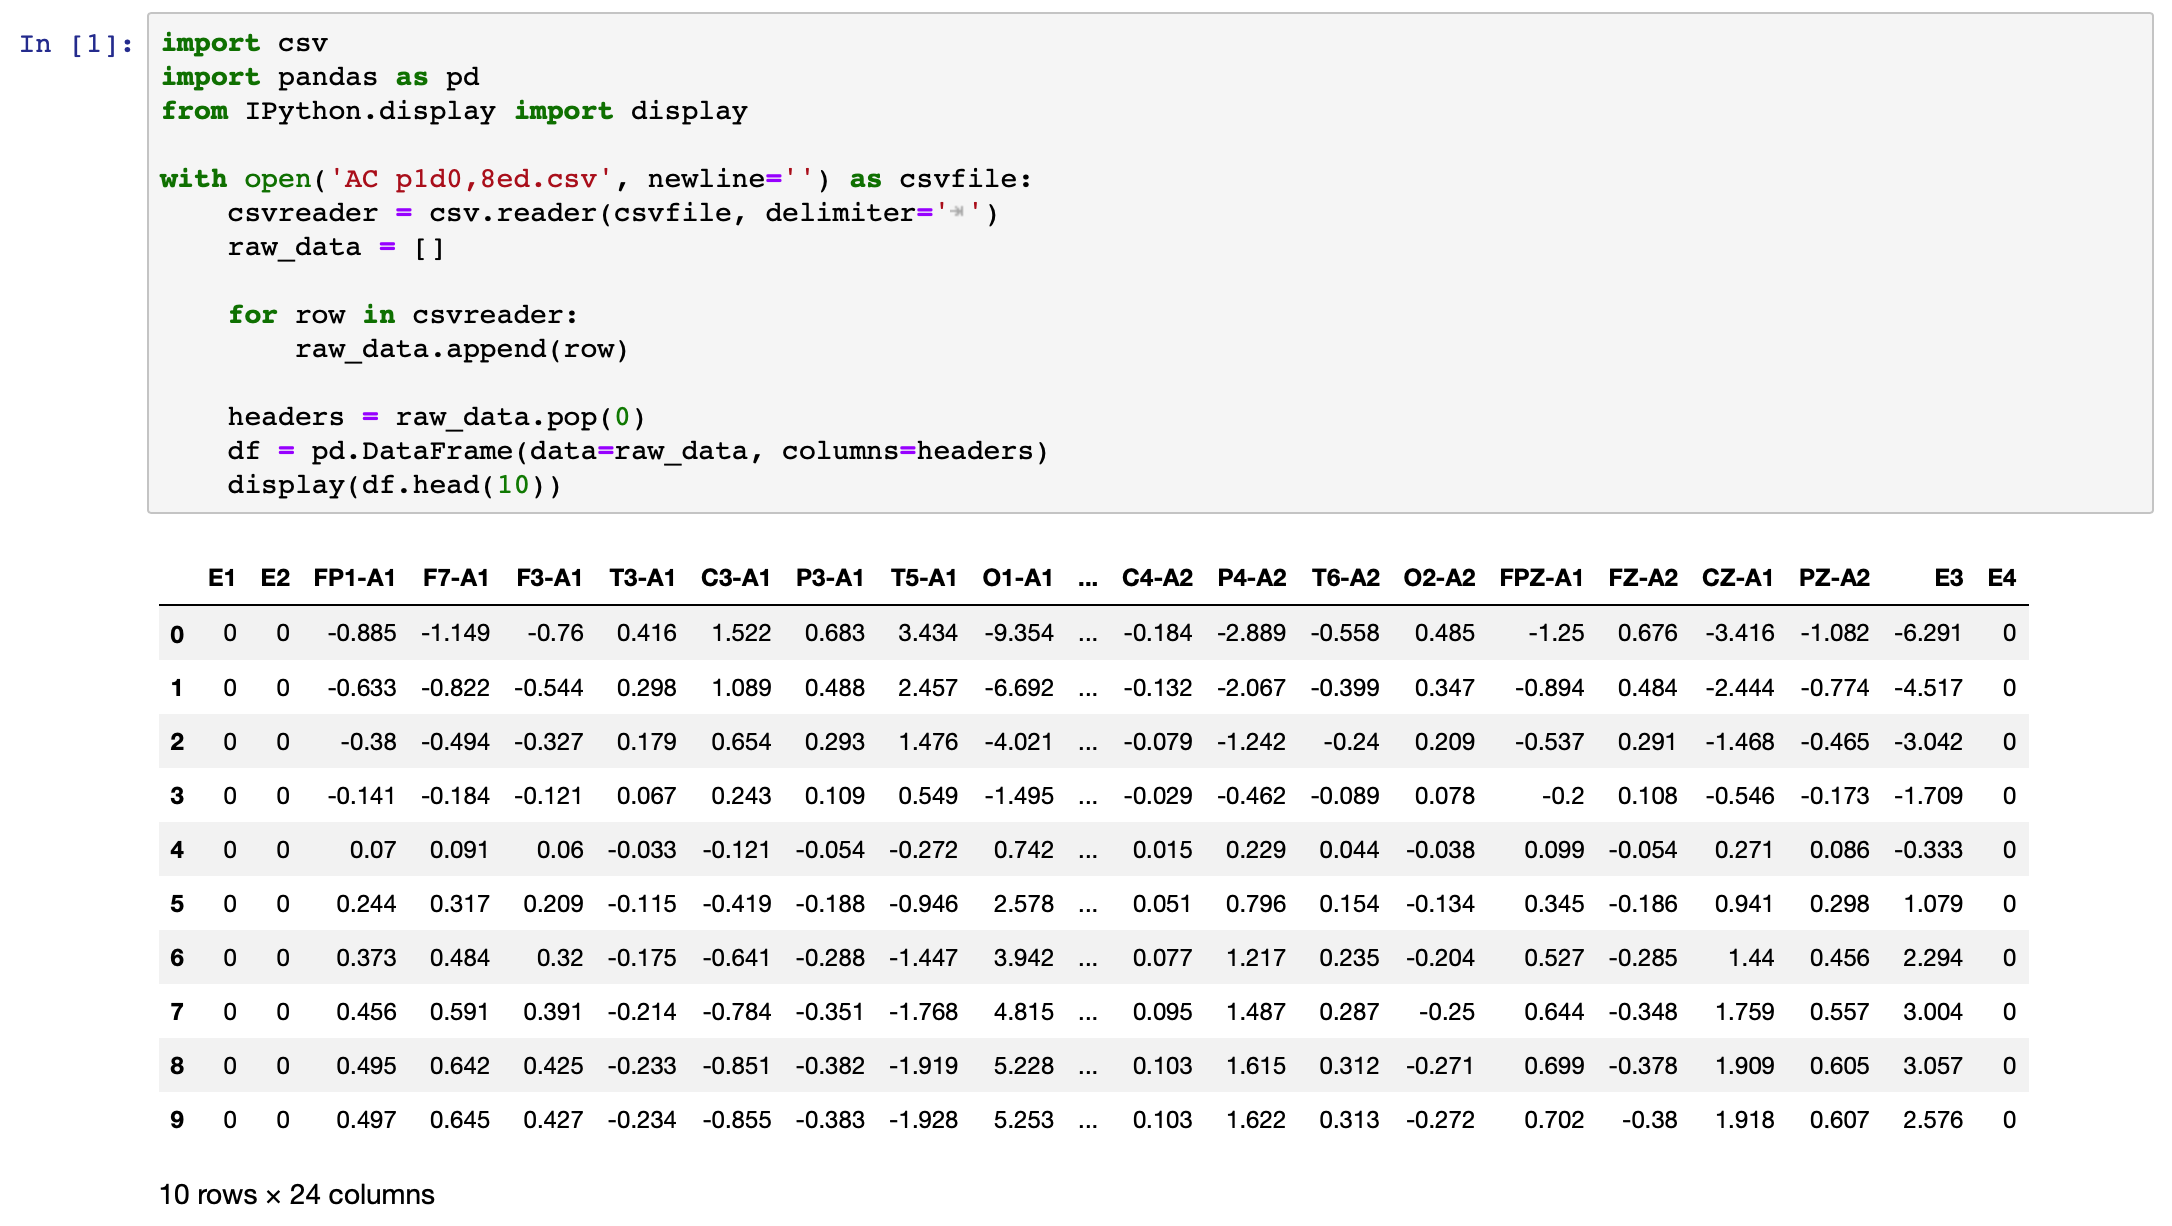
\includegraphics[scale=0.23]{1.png}
  \end{figure}
\end{frame}

\begin{frame}{Ход работы (2/5)}
  \begin{itemize}
      \item {
        Алгоритм написан на языке \texttt{python3.6} с использованием \texttt{Jupyter Notebook}.
      }
      \item {
        При написании алгоритма использованы модули \texttt{pandas} для работы с таблицами, \texttt{numpy} для работы с массивами данных, \texttt{matplotlib} для визуализации графиков.
      }
  \end{itemize}
\end{frame}

\begin{frame}{Ход работы (3/5)}
  Преобразование входных данных и представление их в качестве независимых временных рядов.
  \begin{figure}[h!]
    \centering
    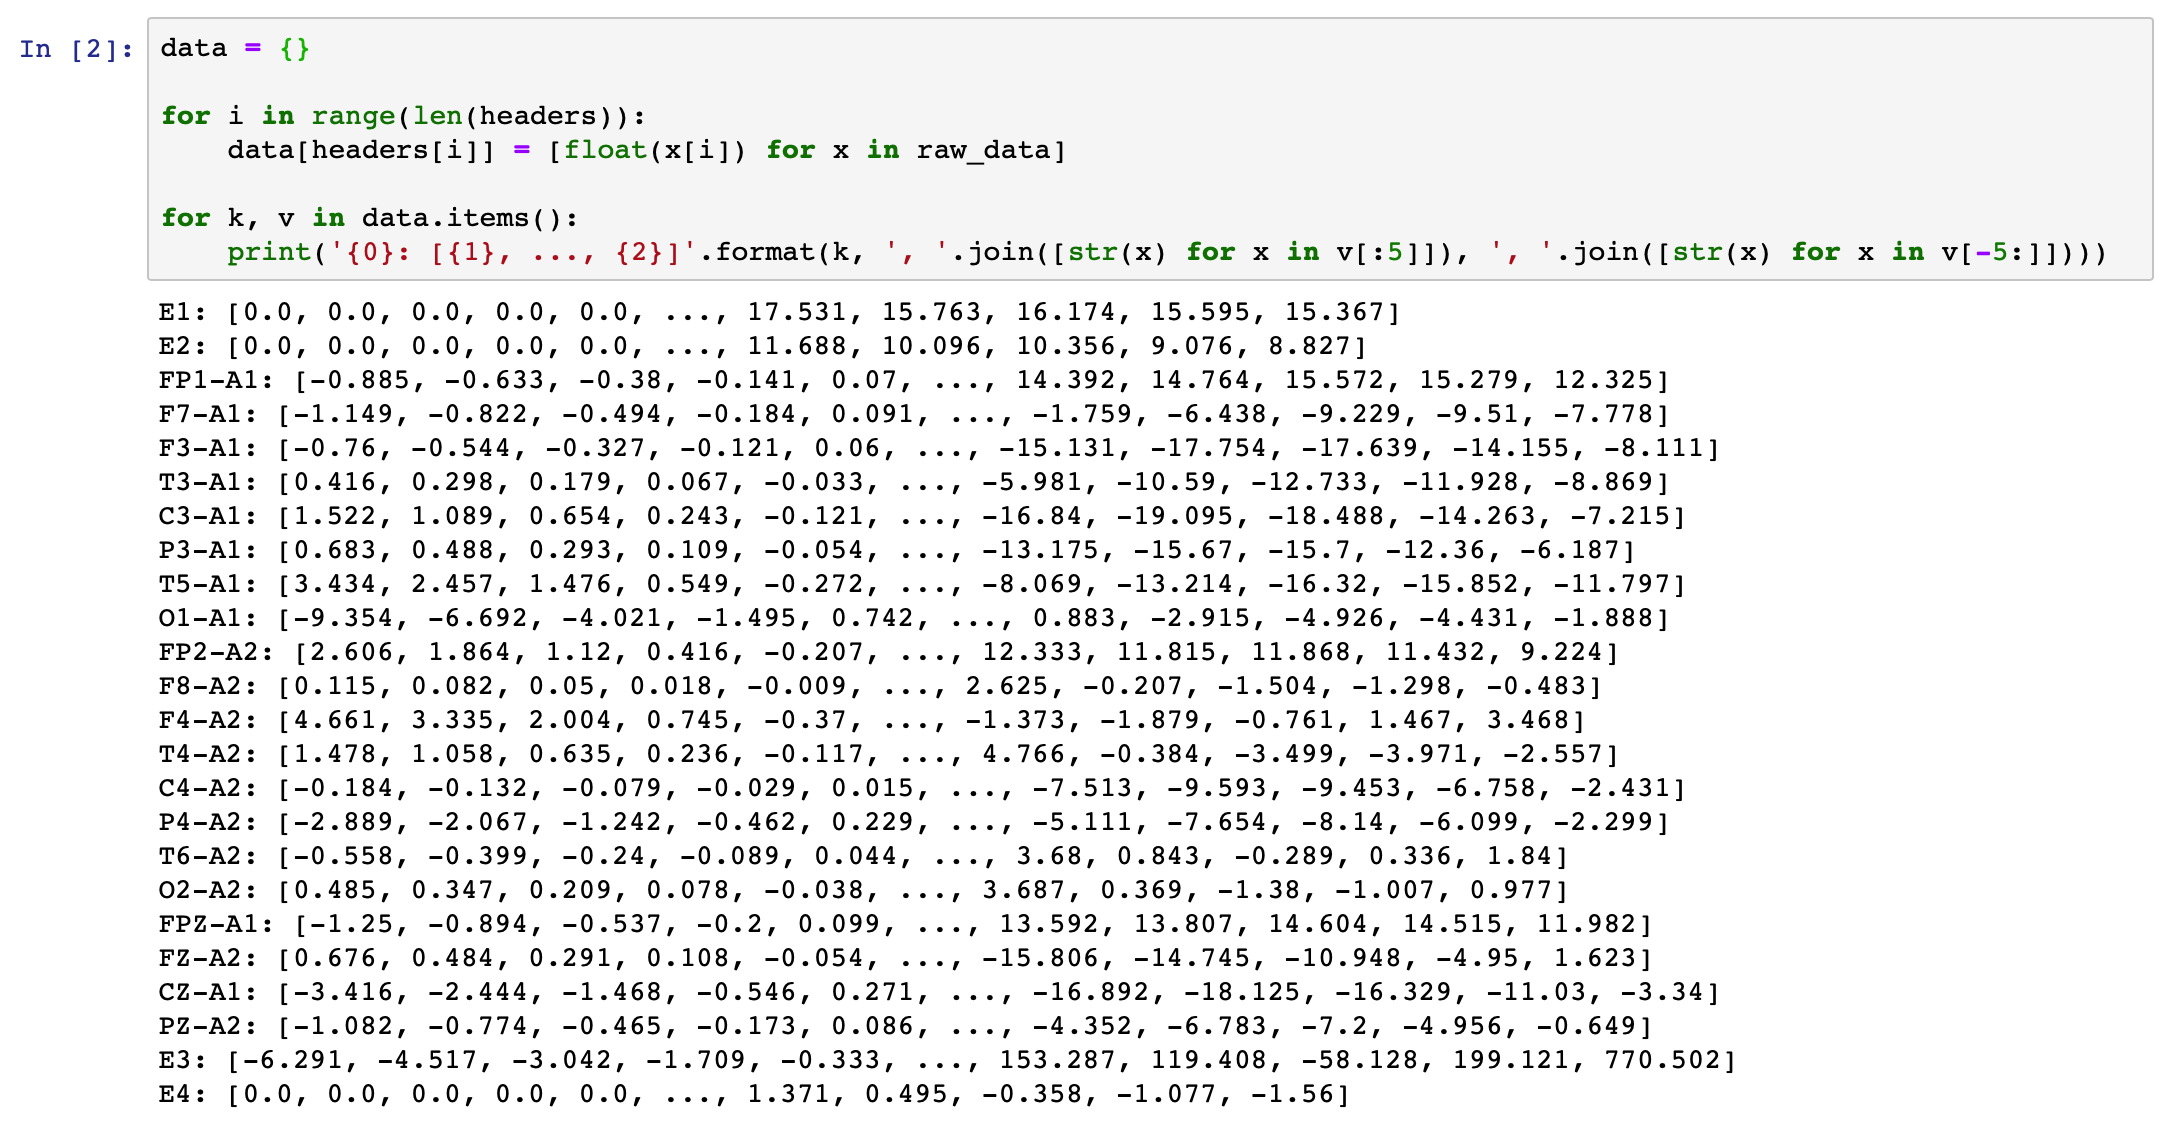
\includegraphics[scale=0.23]{2.png}
  \end{figure}
\end{frame}

\begin{frame}{Ход работы (4/5)}
  Представление одного из временных рядов (на графике каждое 1000-е показание).
  \begin{figure}[h!]
    \centering
    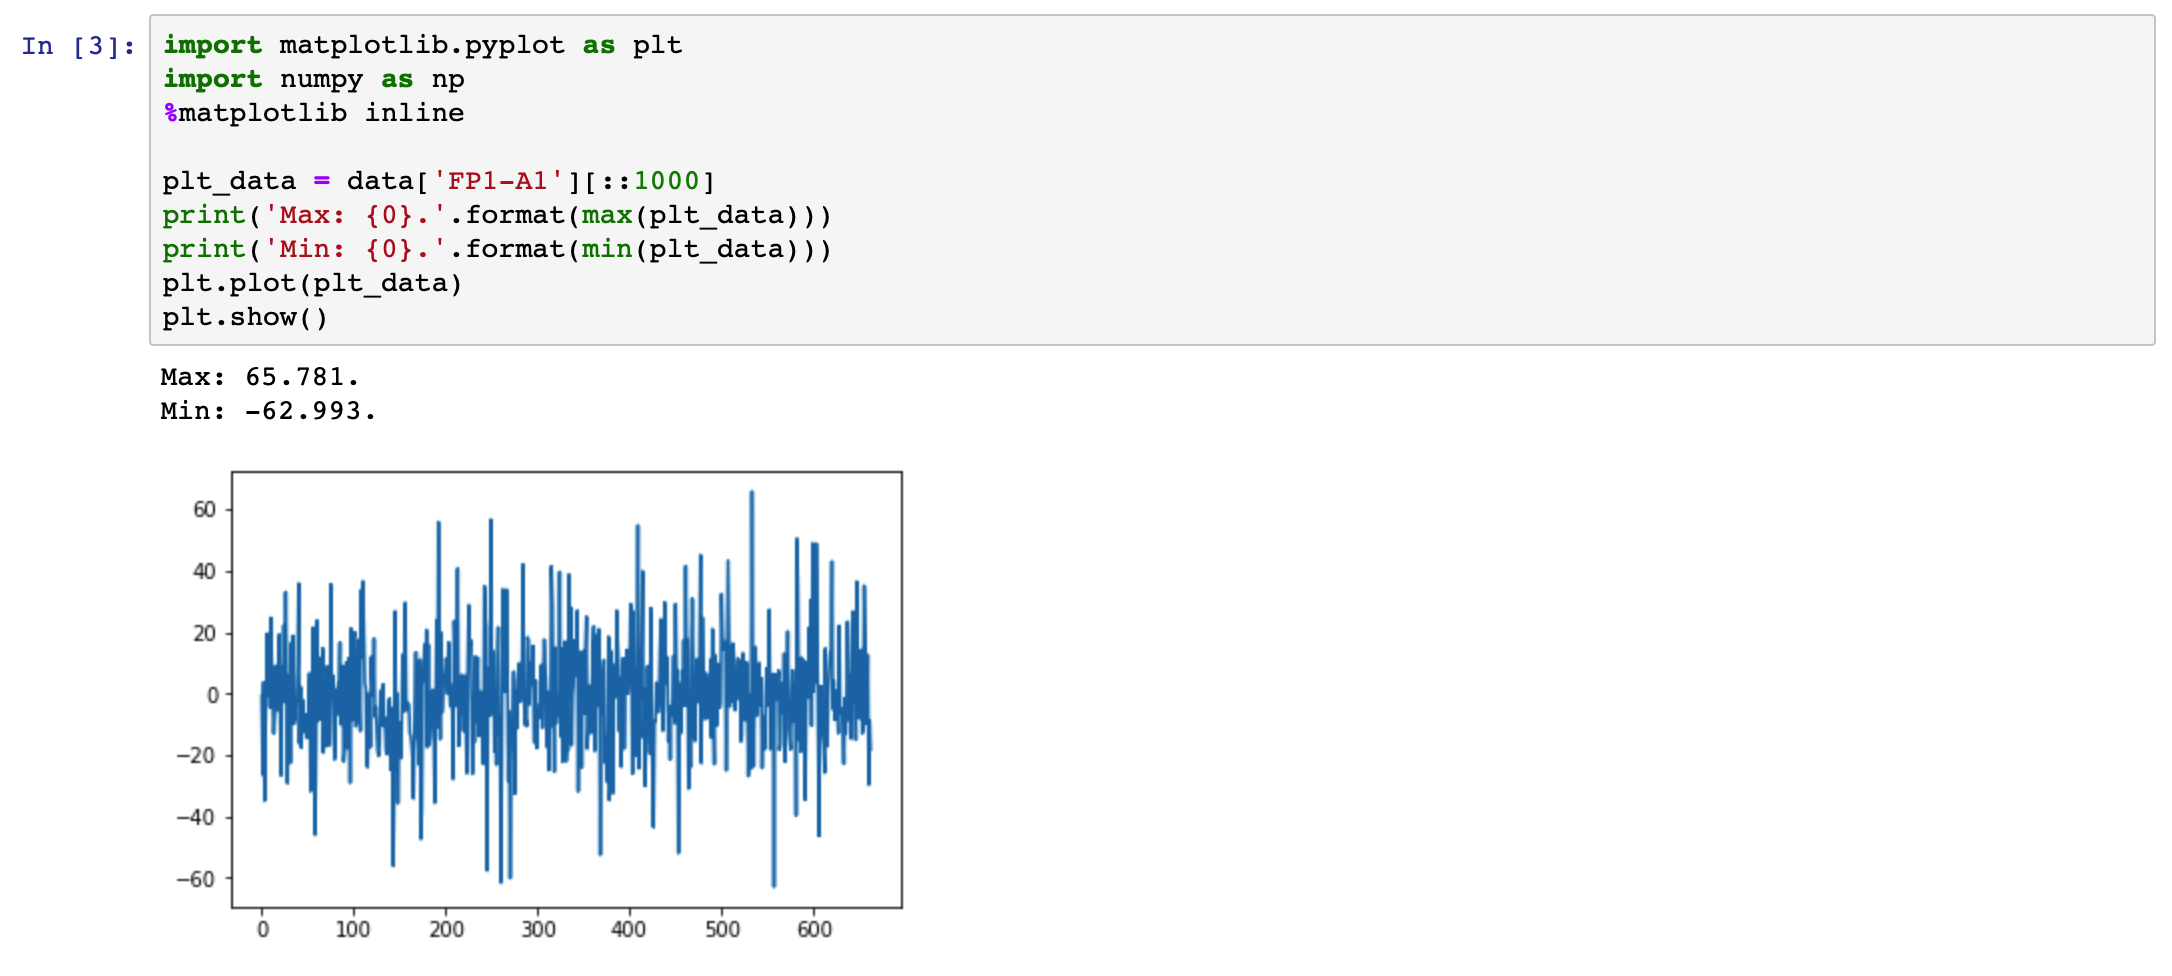
\includegraphics[scale=0.3]{3.png}
  \end{figure}
\end{frame}

\begin{frame}{Ход работы (5/5)}
  \begin{itemize}
      \item {
        Разбиение временных рядов на $n$ равных отрезков (для различных $n \in [10^3; 10^4]$, построение выборочных функций распределения (ВФР) $F_n(x, t_k)$.
      }
      \item {
        Нахождение значения функции $\rho_k = \max_x{|F_n(x,t_k) - F_n(x,t_{k+1}|}$ для того, чтобы понять, стационарен ряд в некотором приближении или нет.
      }
  \par
  \textbf{Дальнейшие планы:}
  \par
  Опираясь на полученные результаты, попытаться построить предиктор эпилептического приступа.
  \end{itemize}
\end{frame}

\begin{frame}
\begin{center}
  \Huge{Спасибо за внимание!}
\end{center}
\end{frame}

\end{document}


